\section{FSMd implementation}
\subsection{Analysis and Design}
Examining the vending machine specification reveals the need for the following components

\begin{itemize}
    \item A clock generator that can generate a 763Hz clock from the 50MHz onboard clock and switch between this clock and a manual one.
    \item An input synchronizer.
    \item The actual vending machine controller. Consisting of a datapath and it's controller.
    \item A 7-segment display driver for the multiplexed 7-segment display on the Basys2 board.
\end{itemize}

These components are also given in the exercise manual and their interconnections can be seen on figure \ref{vending_top}.

\begin{figure}[h]
    \center
    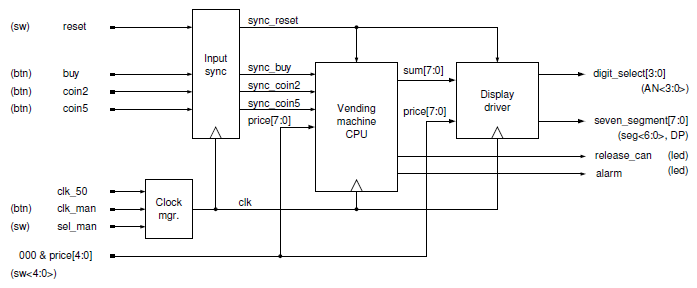
\includegraphics{pictures/vending_top.png}
    \caption{Top level diagram of the vending machine controller, from the exercise manual}
    \label{vending_top}
\end{figure}

Since the inputsynchronizer and clock manager modules have already been given as part of the exercise. The design of those modules will not be covered.

\subsubsection{Display Driver}
The display driver for the vending machine controller, as seen on figure \ref{vending_top}, takes two 8-bit binary numbers
and displays them as hexadecimal on the four 7-segment displays available on the Basys2 board.
However, since we have chosen to display numbers in decimal, we have reduced the size of the input numbers to 7 bits.
This change pervades through the entire design, and therefore the machine is now limited to a max \textbf{sum} of 127.
This should not cause problems however, since reaching this number is deemed unrealistic.
The same change has been made for the \textbf{price} input, but the specification states that this signal is already a 5-bit signal and so the change is without effect. \\
Should the \textbf{sum} exceed 99, we have chosen to let the display show FF.

\paragraph{Display Multiplexing}
Since the 7-segment displays on the Basys2 board have shared cathodes, it is necessary to multiplex the display in order to show 4 different figures.
When this is done with the convenient clock frequency of 763Hz, the display flashes so fast,
that to the human eye, it looks like all the displays are lit at the same time.
This is accomplished by creating a small cyclic FSM with 4 states and a 4-bit output. When this is connected as shown in figure \ref{display_sch},
the outputs will realise the timing diagram shown in figure \ref{display_timing}.
\begin{figure}
    \center
    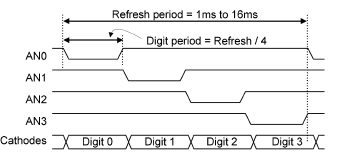
\includegraphics{pictures/display_timing.png}
    \caption{Timing diagram of the display driver FSM, from the exercise manual}
    \label{display_timing}
\end{figure}

Note that the SegmentMultiplexer entity treats input numbers as hexadecial, and so conversion to decimal is handled elsewhere.
This yields a display driver which is a slightly modified form of the circuit presented in figure 5 in the exercise manual.

\begin{figure}
    \center
    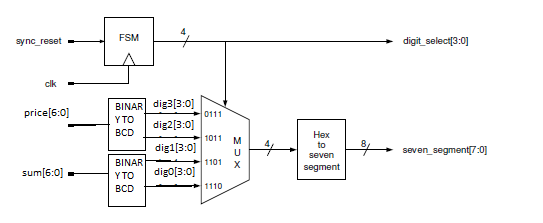
\includegraphics{pictures/display_sch.png}
    \caption{Design of the display driver module from figure \ref{vending_top}}
    \label{display_sch}
\end{figure}

\paragraph{Hexadecimal to BCD conversion}
The BINARY TO BCD modules in figure \ref{display_sch} convert binary numbers to binary coded decimal, using a lookup table.
Since the lookup table is sizeable, it is generated by a java program.
\subsubsection{Vending Machine CPU}
The CPU at the heart of the vending machine takes input from the outside world and keeps track of the various variables the machine operates from. 
Such as the \textbf{sum}. It also directly asserts the \textbf{release\_can} and \textbf{alarm} signals. 

\begin{figure}
    \center
    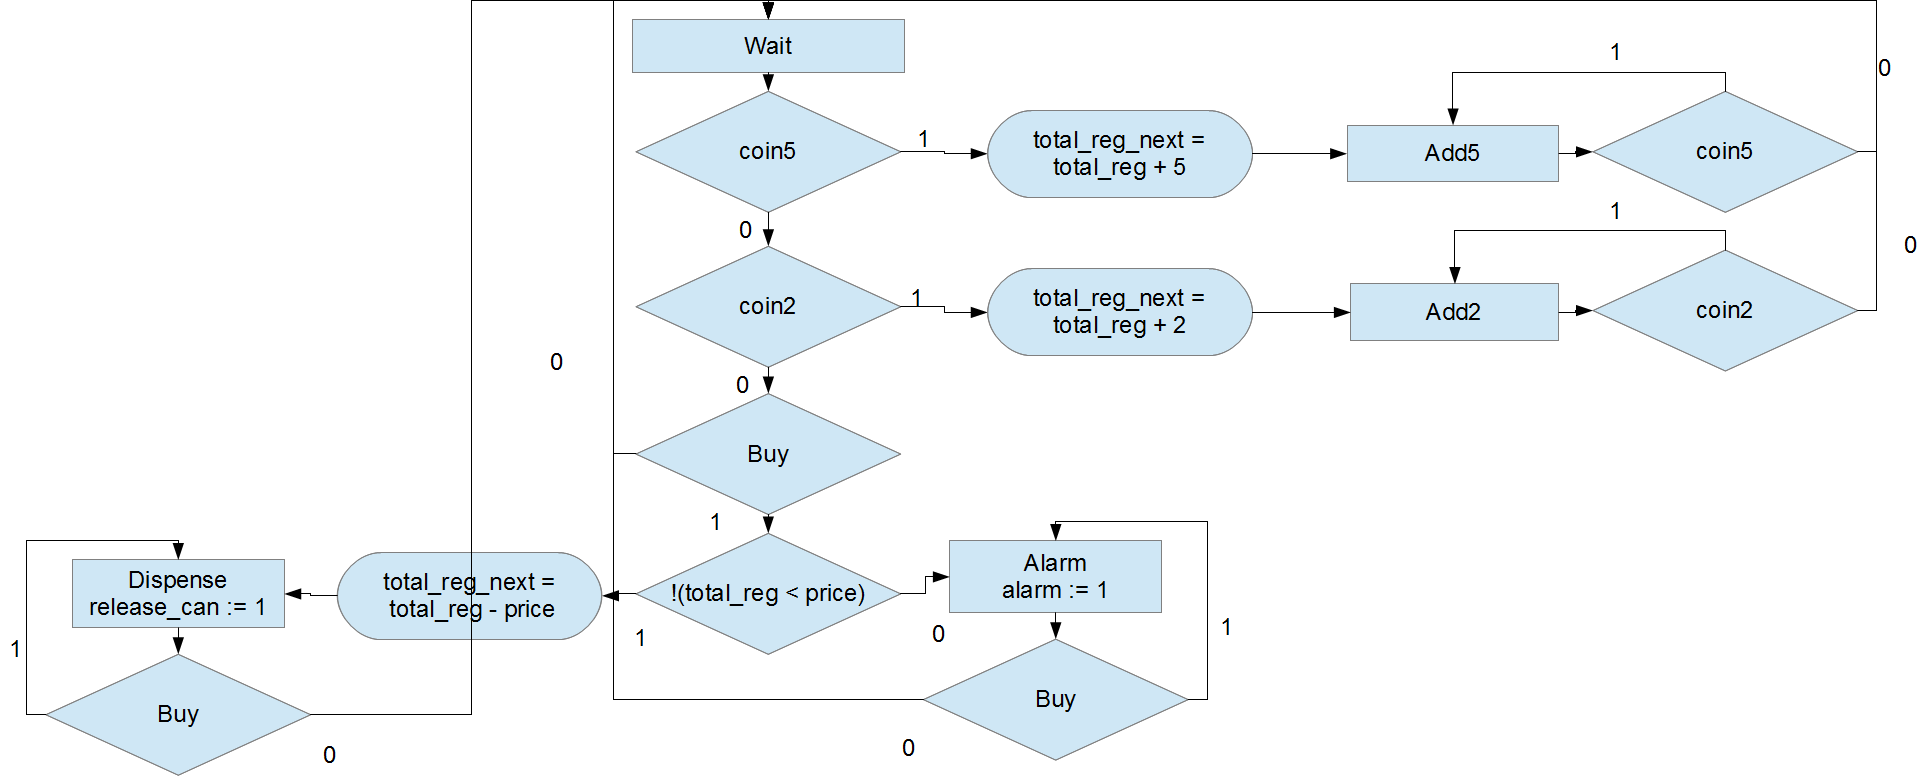
\includegraphics[scale=0.3]{pictures/cola_asm.png}
    \caption{Asm chart for the vending machine cpu, the register containing the \textbf{sum} is called \textbf{total\_reg}}
    \label{cola_asm}
\end{figure}
In accordance with the specification, the asm chart seen in figure \ref{cola_asm}
describes the operation of the vending machine cpu. The Mealy-outputs seen on the asm chart cannot cause metastability since the inputs are synchronized.
Our FSMd implementation of the vending machine controller only needs to keep track of one value, the \textbf{sum}.
This means that the datapath will only need a single register, since the \textbf{price} is an input and not a stored value.
Along with this, the datapath needs to be capable of doing the following operations, as seen on the asm chart. \\


\begin{itemize}
    \item Add 2 and 5 to the \textbf{sum} register
    \item Compare the \textbf{sum} register and \textbf{price}
    \item Subtract the \textbf{price} from the \textbf{sum}
\end{itemize}

The datapath seen in figure \ref{fsmd_datapath} meets all of these requirements.
\begin{figure}
    \center
    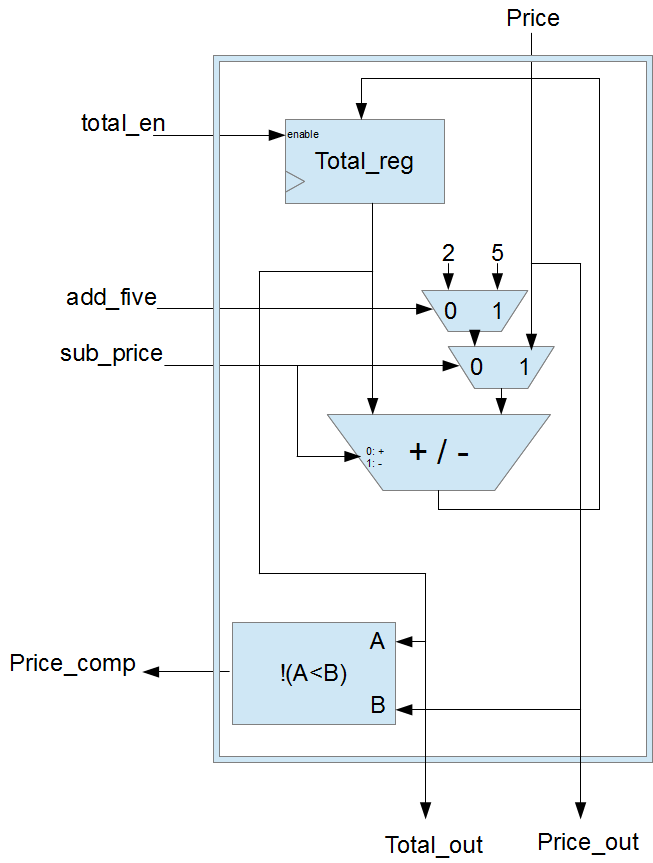
\includegraphics[scale=0.5]{pictures/datapath_cola.png}
    \caption{Datapath for the vending machine FSMd}
    \label{fsmd_datapath}
\end{figure}

To control the datapath, an FSM is needed. This FSM has the same states as
shown in the ASM chart, but it's outputs are logic signals instead of complex operations.
An FSM that, in conjuction with the datapath realises the ASM chart in figure \ref{cola_asm}, can be seen in figure \ref{cola_fsm}.

\begin{figure}
    \center
    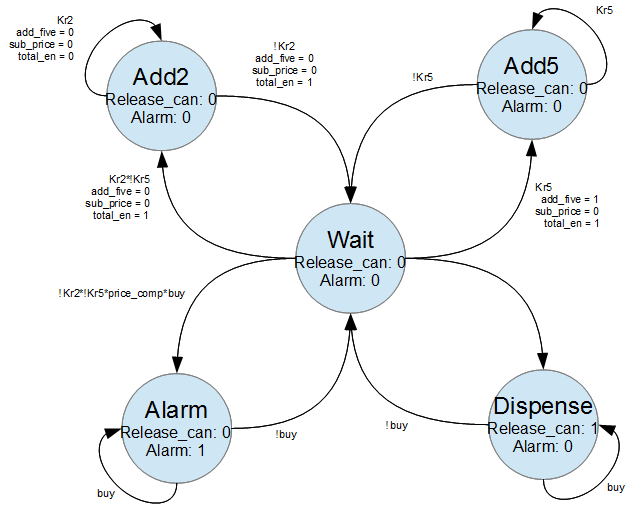
\includegraphics[scale=0.5]{pictures/fsm1_cola.png}
    \caption{FSM controller of the datapath seen in figure \ref{fsmd_datapath}}
    \label{cola_fsm}
\end{figure}


